\documentclass[8pt,landscape]{article}

% PACKAGES
\usepackage[letterpaper, margin=0.1in]{geometry}
\usepackage{amsmath, amssymb, geometry}
\usepackage{multicol}
\usepackage{setspace}
\usepackage{sectsty}
\usepackage{verbatim}
\usepackage{graphicx}
\usepackage{xcolor}
\usepackage{listings}
\usepackage{enumitem}
\usepackage{booktabs} % For better tables if needed

% Define a custom color for code highlighting and environment
\definecolor{myred}{RGB}{204, 0, 0} % A strong red
\definecolor{mygray}{RGB}{240, 240, 240} % Light gray for background

% LISTINGS SETUP for R and Python
\lstset{
  basicstyle=\ttfamily\scriptsize\color{black}, % Tiny font for code
  backgroundcolor=\color{mygray},
  frame=single,
  frameround=tttt,
  framesep=3pt,
  rulesepcolor=\color{black!20},
  breaklines=true,
  columns=fullflexible,
  showstringspaces=false,
  commentstyle=\color{gray},
  keywordstyle=\color{blue!80!black},
  stringstyle=\color{myred}, % Use red for strings to match the custom \code{} style
  breakatwhitespace=true,
  xleftmargin=0pt,
  xrightmargin=0pt,
  aboveskip=0.5ex,
  belowskip=0.5ex
}

% FORMATTING
\setstretch{0.9} % Reduce line spacing
\setlength{\parindent}{0pt}
\setlength{\parskip}{0pt}

% Reduce section spacing and change color
\sectionfont{\fontsize{8}{9}\selectfont\bfseries\color{black}} % Main section font: 8pt
% Reduce subsection spacing and make subsections blue
\makeatletter
\renewcommand{\subsection}{\@startsection{subsection}{2}{0pt}%
    {0.1ex}% space before subsection
    {0.1ex}% space after subsection
    {\fontsize{8}{9}\bfseries\color{blue}}} % Subsection font: 8pt
\makeatother

% Custom command for red-highlighted code/commands (for in-line use)
\newcommand{\code}[1]{\textcolor{myred}{\texttt{#1}}}

% Custom small text wrapper - ensuring 8pt for body text
\newcommand{\smalltext}[1]{%
  {\fontsize{8}{9}\selectfont\sloppy #1\par}%
}

% DOCUMENT START
\begin{document}
\fontsize{8}{9}\selectfont % Set the base font size to 8pt and line skip to 9pt for the entire document
\pagestyle{empty}
\begin{multicols}{3}

\subsection{General Structure}
\begin{lstlisting}[language=Python]
  rating_density = alt.Chart(df, title="Title").transform_density(
    density='col',
    groupby=['col2'],
    as_=['col', 'density']
).mark_area(
    opacity=0.6,
    line={'color': 'white'}
).encode(
    x=alt.X('col1:Q',
            title='the value',
            scale=alt.Scale(domain=[0, 10000]),
            axis=alt.Axis(format='~s',grid=False,tickCount=10)),
    y=alt.Y('density:Q',
            title='density',
            scale=alt.Scale(domain=[0, 0.000100]),
            axis=alt.Axis(format='.6f',grid=False)).stack(False),
    color=alt.Color('where:N',
                    scale=alt.Scale(
                        domain=['My state', 'Neighboring states'],
                        range=['#A0D2E8', '#A0E8AF']
                    ),
                    legend=alt.Legend(
                        orient='top' 
                    )
                   )
).properties(
    width=600,
    height=400
)
\end{lstlisting}
\begin{lstlisting}[language=R]
  options(repr.plot.width=7, repr.plot.height=3)

chart <- ggplot(wages) +
    aes(
        x = salary,
        y = when,
        fill = when
    ) +
    geom_violin() +
    geom_point(stat = 'summary', fun = median, color = 'White') +
    geom_point(stat = 'summary', fun = mean, color = 'Black') +
    labs(
        x = "Worker Salary ($)",
        y = "When",
        title = "Salary Distribution Before and After Policy Implementation" 
    ) +
    scale_x_continuous(
        limits = c(10, 40), oob = scales::oob_keep,
                labels = scales::dollar_format(), 
    ) 
chart
\end{lstlisting}

\subsection{HEAT MAPS}
\smalltext{
A 2D histogram is a type of heatmap, where count is mapped to color, you could also have used a mark that maps size to color, which might even be more effective but that is not as commonly seen.
}
\begin{lstlisting}[language=Python]
alt.Chart(df).mark_rect().encode(alt.X('col1').bin(maxbins=40),
alt.Y('col2').bin(maxbins=40),alt.Color('count()')
)
\end{lstlisting}
\smalltext{
    Instead of squares,\textbf{hexagonal bins} can be used. These have theoretically superior qualities over squares, such as a more natural notation of neighbors. \\
    2 dimensional \textbf{KDEs} in ggplot. This works just like 1D KDEs, except that the kernel on each data point extends in 2 dimensions \\
    Use \textbf{ridges contours}, similar to a topographic map. These contour plots are often less intuitive than the density plot above, so the recommendation is to use the density plot instead.
}
\begin{lstlisting}[language=R]
ggplot(df) + aes(x = col1, y = col2) + geom_bin2d() or geom_hex() or  geom_density_2d_filled() or geom_density_2d()
\end{lstlisting}

\subsection{AXIS LABEL FORMATTING}
\smalltext{
\textbf{Scientific Notation \& Grid Tick Modifications} \\
Scientific notation, Consider formatting axis labels using plain numbers or appropriate unit prefixes (e.g., thousands, millions, micro, milli) to improve readability. \\[6pt]
Note that \texttt{tickCount} cannot be applied to binned data, so the plot has been adjusted here to demonstrate its effect.
}

\begin{lstlisting}[language=Python]
.alt.X('col').axis(format='e') # For e like notation
.alt.X('col').axis(format='s') # Standard international (SI) units
.alt.X('col').axis(format='~s') # Removes trailing zeros
.alt.X('col').axis(format='\$~s') # Formaters can also be combined.
.alt.X('col').axis(format='.1%') # Decimal formats
.alt.X('col').axis(None) #Remove an axis altogether
.alt.Y('col').axis(tickCount=2) #ticks on axis
.alt.Y('col').axis(grid=False) #Remove grid
.alt.Y('col').sort('-y') #Sort y axis
alt.Y('coly').bin(maxbins=400).scale(domain=[0, 2000]), #Set scale
alt.themes.enable('dark') #Dark theme scale
alt.Color('count()').legend(None) # remove a legend 
alt.Y('coly').bin(maxbins=400).scale(domain=(0, 2000), reverse=True), #Reversing an axis
alt.Y('col:Q',bin=alt.Bin(maxbins=20),
        title='Y Label', #Set Label
        axis=alt.Axis(format='.1%', titleFontSize=14, labelFontSize=12))
\end{lstlisting}
\begin{lstlisting}[language=R]
ggplot(df) + aes(x = colx,y = coly) + geom_hex() +
  guides(fill = "none") # remove a legend 
  scale_x_continuous(
    labels = scales::label_dollar(scale = .001, suffix = "K"),
    labels = scales::label_number(scale_cut = scales::cut_si('')),
    limits = c(10, 31), oob = scales::oob_keep, #scale limit
    limits = c(2000, 0), trans = 'reverse', #reversing an axis
    labels = scales::label_dollar(), #label formater
    breaks = scales::pretty_breaks(n = 10) #tick count
  )
\end{lstlisting}
\begin{lstlisting}[language=R]
ggplot(df) + aes(x = col1, y = col2) + geom_hex() +
  labs(
    x = 'col1',
    y = 'col2',
    title = 'title',
    subtitle = 'subtitle'
  )
\end{lstlisting}

\subsection{Trendlines - Mean Line}
\smalltext{
Trendlines (also sometimes called “lines of best fit”, or “fitted lines”) are good to highlight general trends in the data that can be hard to elucidate by looking at the raw data points. This can happen if there are many data points or many groups inside the data.
}
\begin{lstlisting}[language=Python]
points + points.mark_line().encode(y='mean(Horsepower)')
\end{lstlisting}
\begin{lstlisting}[language=R]
ggplot(cars) + aes(x = Year, y = Horsepower, color = Origin) +
  geom_point() + geom_line(stat = 'summary', fun = 'mean')
\end{lstlisting}
\subsection{Trendlines - Regression Lines}
\smalltext{
If you want an easy-to-interpret trend line, use a rolling mean 
(or a simple mean if the data isn’t too noisy). It naturally 
highlights patterns as we would notice them visually and requires fewer 
statistical assumptions than methods like \textbf{linear regression}. 
}
\begin{lstlisting}[language=Python]
points +  points.mark_line(size=3).transform_regression(
    'Year',
    'Horsepower',
    groupby=['Origin'],
    method='poly' #for regression line that is quadratic, polynomial
)
\end{lstlisting}

\subsection{Trendlines - loess/lowess Lines}
\smalltext{
Where the w stands for “weighted”. You can fit multiple equations (usually linear and quadratic) to smaller subsets of the data, and add them together to get the final line. 
\textbf{bandwidth} parameter controls how much the loess fit should be influenced by local variation in the data, similar to the effect of the bandwidth parameter for a KDE.
bandwidth of 1 corresponds to using all the data and will be similar to a linear regression
}
\begin{lstlisting}[language=Python]
points +  points.mark_line(size=3).transform_loess(
    'Year',
    'Horsepower',
    groupby=['Origin'],
    bandwidth=0.8 #optional param
)
\end{lstlisting}
\begin{lstlisting}[language=R]
ggplot(cars) + 
    aes(x = Year,
        y = Horsepower,
        color = Origin,
        fill = Origin) + #color the confidence interval the same as the lines.
    geom_point() +
    geom_smooth() #Introduce CI
    geom_smooth(se = FALSE, size = 2, span=1) #Introduce bandwidth use span
    geom_smooth(se = FALSE, size = 2, method = 'lm') #linear regression instead of loess
\end{lstlisting}
\subsection{When to choose which trendline:}
\begin{itemize}
    \item \textbf{Rolling mean / mean:} Best for clear, easy-to-read trends and general audiences. Simple and intuitive, but not suitable for predictions beyond your data.
    \item \textbf{Linear (or similar model):} Use when your data follows a clear equation. Good for showing consistent patterns and making predictions outside your data range.
    \item \textbf{Loess (or smooth curve):} Ideal for showing natural, flexible trends in current data without assuming a strict model, though poor for extrapolation.
\end{itemize}

\subsection{Color schemes/maps:}
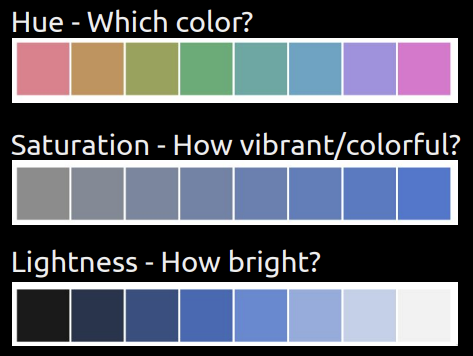
\includegraphics[width=0.5\linewidth, height=2cm]{HSL.png}
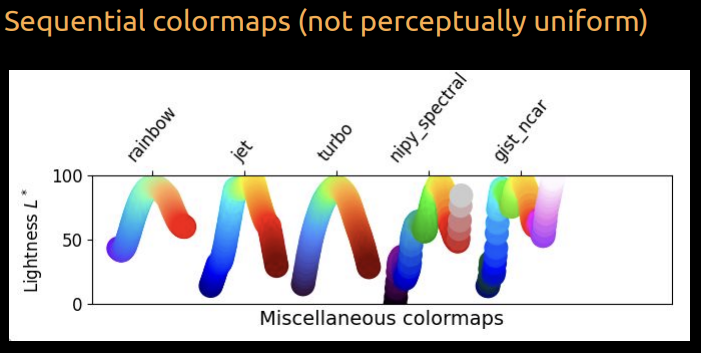
\includegraphics[width=0.5\linewidth, height=2cm]{seq-not.png}
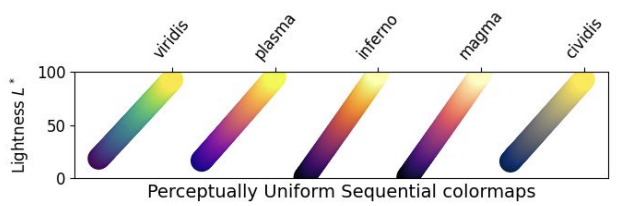
\includegraphics[width=0.5\linewidth, height=2cm]{seq.png}
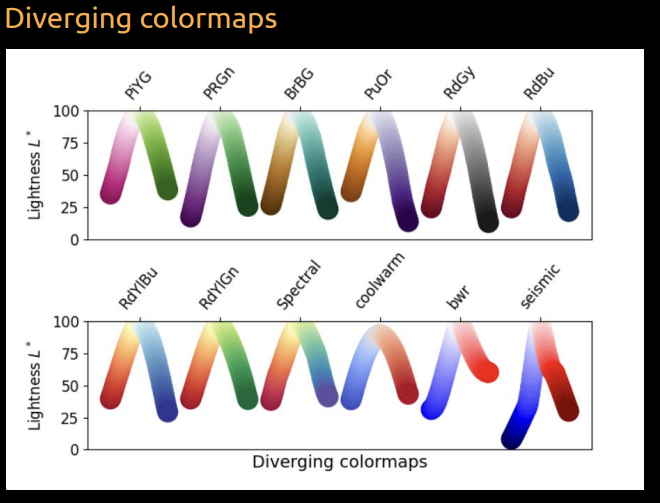
\includegraphics[width=0.5\linewidth, height=2cm]{diverge.png}
\smalltext{
colormap is useful for (categorical, sequential, diverging, cyclic) \\
\textbf{Categorical:} Single color for each category \\
\textbf{Sequential:} Shades of a color \\
}
\begin{lstlisting}[language=Python]
#Sequential
alt.Chart(iris).mark_circle(size=100).encode(
    x='petalWidth',
    y='petalLength',
    color=alt.Color('petalWidth').scale(scheme='viridis', reverse=True)
)
#Diverging has a natural midpoint, 
# such as a correlation that is defined from -1 to 1
corr_df = data.gapminder().corr(numeric_only=True).stack().reset_index(name='corr')
alt.Chart(corr_df).mark_rect().encode(
    x='level_0',
    y='level_1',
    tooltip='corr',
    color=alt.Color('corr').scale(domain=(-1, 1), scheme='purpleorange')
).properties(
    width=200,
    height=200
)
\end{lstlisting}
\begin{lstlisting}[language=R]
#Sequential
ggplot(iris) + 
    aes(x = Petal.Width,
        y = Petal.Length,
        color = Petal.Width) +
    geom_point(size = 5) +
    scale_color_viridis_c()
#Diverging has a natural midpoint, 
# such as a correlation that is defined from -1 to 1
ggplot(corr_df) +
    aes(x = level_0,
        y = level_1,
        fill = corr) +
    geom_tile() +
    ggthemes::scale_fill_gradient2_tableau()
\end{lstlisting}

\subsection{Direct labeling instead of using a legend}
\begin{lstlisting}[language=Python]
lines = alt.Chart(stocks).mark_line().encode(
    x='date',
    y='price',
    color=alt.Color('symbol').legend(None)
)
text = alt.Chart(stock_order).mark_text(dx=20).encode(
    x='date',
    y='price',
    text='symbol',
    color='symbol'
)
lines + text
\end{lstlisting}
\begin{lstlisting}[language=R]
ggplot(stocks) + 
    aes(x = date,
        y = price,
        color = symbol,
        label = symbol) +
    geom_line() +
    geom_text(data = stock_order, vjust=-1) +
    ggthemes::scale_color_tableau() +
    theme(legend.position = 'none')
\end{lstlisting}

\subsection{Confidence Intervals}
\begin{lstlisting}[language=Python]
points.mark_errorband(extent='ci') + points.encode(y='mean(Horsepower)').mark_line() #add meanline with CI
err_bars = alt.Chart(cars).mark_errorbar(extent='ci', rule=alt.LineConfig(size=2)).encode(
    x='Horsepower',
    y='Origin'
)
(err_bars.mark_tick(color='lightgrey')
 + err_bars
 + err_bars.mark_point(color='black').encode(x='mean(Horsepower)'))
\end{lstlisting}
\begin{lstlisting}[language=R]
ggplot(cars) + aes(x = Year,y = Horsepower,color = Origin,fill = Origin) +
    geom_line(stat = 'summary', fun = mean) +
    geom_ribbon(stat = 'summary', fun.data = mean_cl_boot, alpha=0.5, color = NA)
ggplot(cars) +
    aes(x = Horsepower,y = Origin) +
    geom_violin(color = NA, fill = 'steelblue', alpha = 0.4) +
    geom_pointrange(stat = 'summary', fun.data = mean_cl_boot, size = 0.7)
\end{lstlisting}
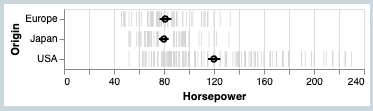
\includegraphics[width=0.5\linewidth, height=2cm]{ci.png}

\subsection{Figure composition}
\begin{lstlisting}[language=Python]
mpg_weight & hp_weight #Concatenate plots vertically
mpg_weight | hp_weight #Concatenate plots Horizontally
plot_grid(hp_weight, mpg_weight) #Concatenate plots Horizontally
plot_grid(origin_count, mpg_weight, ncol=1) #Concatenate plots vertically
alt.Chart(cars).mark_circle().encode(...).interactive() #Panning and zooming
brush = alt.selection_interval()
alt.Chart(cars).mark_circle().encode(...).add_params(brush) #Interval selections
\end{lstlisting}

\subsection{Highlighting points with selections}
\begin{lstlisting}[language=Python]
brush = alt.selection_interval()
alt.Chart(cars).mark_circle().encode(
    x='Horsepower',
    y='Miles_per_Gallon',
    color=alt.condition(brush, 'Origin', alt.value('lightgray'))
).add_params(brush)
\end{lstlisting}

\subsection{Linking selections across plots}
\begin{lstlisting}[language=Python]
brush = alt.selection_interval(resolve='union')  # The default is 'global' #resolve='intersect'
points = alt.Chart(cars).mark_circle().encode(
    x='Horsepower',
    y='Miles_per_Gallon',
    color=alt.condition(brush, 'Origin', alt.value('lightgray'))
).add_params(brush)
points | points.encode(y='Weight_in_lbs')
\end{lstlisting}

\subsection{Click selections}
\begin{lstlisting}[language=Python]
brush = alt.selection_interval()
click = alt.selection_point(fields=['Origin'], on='mouseover')
points = alt.Chart(cars).mark_circle().encode(
    x='Horsepower',
    y='Miles_per_Gallon',
    color=alt.condition(brush, 'Origin', alt.value('lightgray'))
).add_params(brush)
bars = alt.Chart(cars).mark_bar().encode(
    x='count()',
    y='Origin',
    color='Origin',
    opacity=alt.condition(click, alt.value(0.9), alt.value(0.2))
).add_params(click)
points & bars
\end{lstlisting}

\end{multicols}
\end{document}